\documentclass[11pt, a4paper, oneside]{article}

\usepackage[portuguese]{babel}
\usepackage[utf8]{inputenc}
\usepackage{geometry}
\usepackage{booktabs}
  
\geometry{
left   = 30mm,
right = 30mm,
top   = 30mm,
bottom=30mm,
}

\usepackage{color}   %May be necessary if you want to color links
\usepackage{hyperref}
\hypersetup{
    colorlinks=true, %set true if you want colored links
    linktoc=all,     %set to all if you want both sections and subsections linked
    linkcolor=blue,  %choose some color if you want links to stand out
}

\usepackage{tikz}
\usetikzlibrary{shapes,arrows}


\tikzstyle{block} = [draw, fill=blue!20, rectangle, 
    minimum height=3em, minimum width=6em]
\tikzstyle{sum} = [draw, fill=blue!20, circle, node distance=1cm]
\tikzstyle{input} = [coordinate]
\tikzstyle{output} = [coordinate]
\tikzstyle{pinstyle} = [pin edge={to-,thin,black}]




\usepackage{graphicx}

\usepackage{amssymb, amsmath, amsthm}

\title{Relatório de Laboratório de Controle de Sistemas : SEL0328}
\author{Aluno:Fabiano Aparecido Marino \\NºUsp:7143980	\\Pedro Carrascosa \\NºUsp:7173480\\ Professor: Rodrigo Ramos}

\begin{document}

\maketitle

\begin{figure}[h!]
\centering
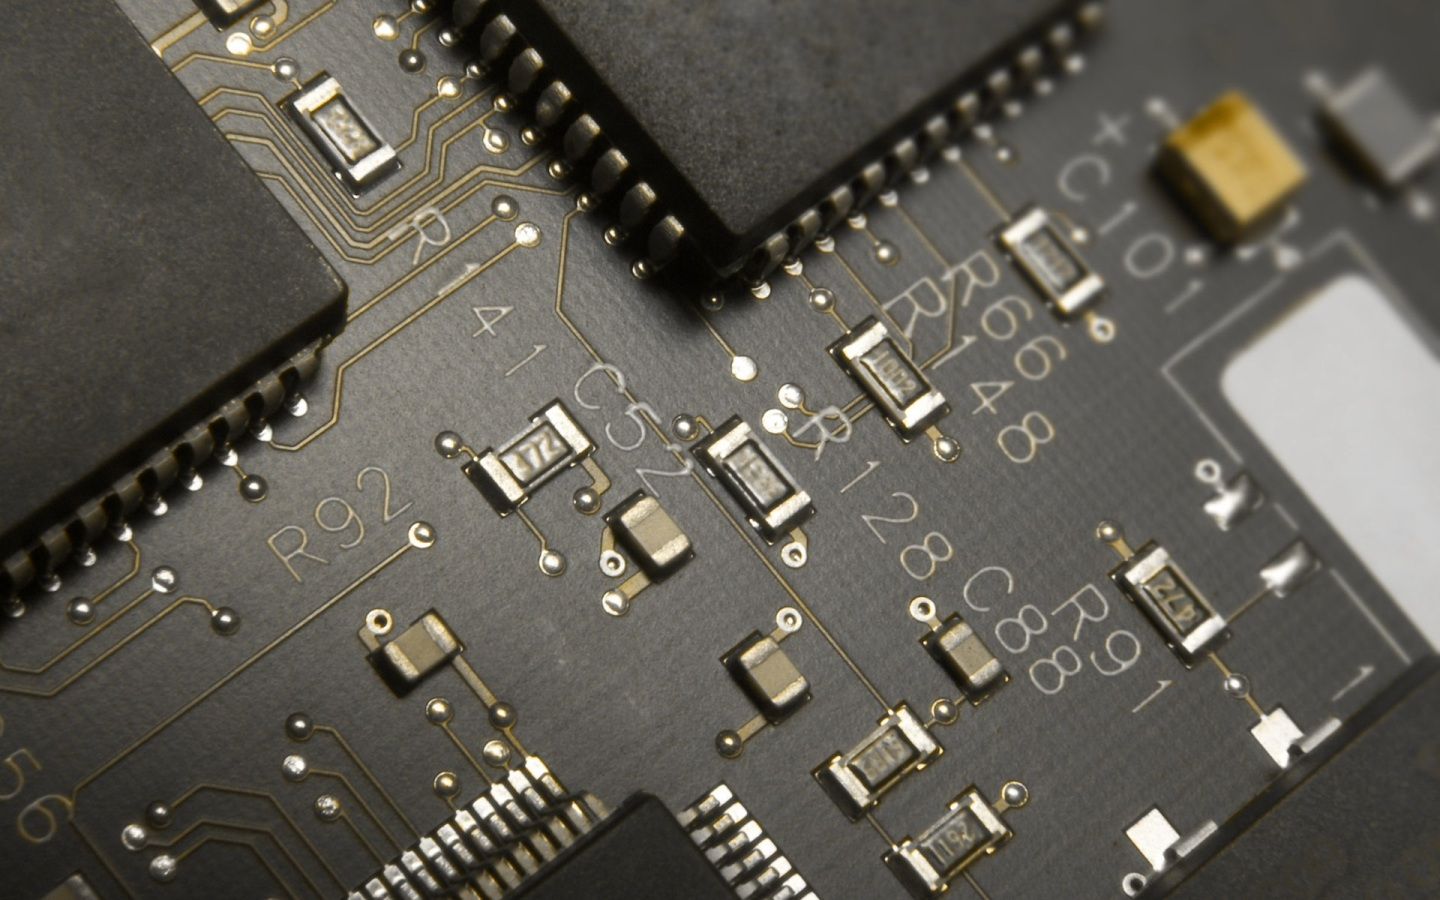
\includegraphics[width=1\linewidth]{capa.jpg}
\end{figure}


\pagebreak

\tableofcontents
\listoffigures

\pagebreak

\section{Introdução}
O presente relatório tem como objetivo apresentar os resultados obtidos na disciplina de Laboratório de Controle de Sistemas, ministrada pelo professor Rodrigo Ramos.O objetivo das práticas realizadas consistem no controle de velocidade de um motor de corrente contínua , sendo que, para isto, busca-se explorar caracteríticas do motor e periféricos, tais como função de transferência do motor, ganho do tacogerador , constante do PWM (Pulse Width Modulation) utilizado, dentre outras discutidas no decorrer do relatório.Os experimentos são verificados via simulação, utilizando o software Matlab-Simulink como simulador.

\subsection{Motor de Corrente Contínua}
A planta utilizada para o controle é um motor de corrente contínua, que consite em uma máquina elétrica que converte energia elétrica em mecânica, na forma de rotação de um eixo.A construção do motor consiste em dois enrolamentos, um que permanece estático, chamado de estator, e outro que se movimenta chamado armadura.Em ambos há a passagem de corrente, afim de gerar um campo magnético, porém, devido a disposição desses elementos, o campo gerado cria um torque fazendo com que haja a rotação da armadura, que por sua vêz, gira um eixo, completando assim a conversao de energia elétrica em mecânica.
\subsection{Tacogerador}
Consiste em um elemento que gera um valor de tensão em relação ao valor de velocidade de rotação do eixo do motor.Seu princípio de funcionamento é o mesmo que máquinas geradoras de energia, ou seja, o movimento mecânico faz com que imãs permantes girem e devido isso altera-se o fluxo de campo magnético em uma bobina, gerando assim um nível de tensão.
\subsection{Optoacoplador}
Consiste em dispositivo também utilizado para se medir a velocidade em motores ou elementos girantes, porém seu funcionamento não é magnético, mas sim optico, sendo que, quanto maior a velocidade, maior o número de pulsos que o optoacoplador emite, havendo uma relação entre a frequência da onda quadrada gerada e velocidade de rotação do motor.Este dispositivo fio utilizado para obter-se o ganho do tacogerador, afinal, sem este, fica impossível utilizá-lo, ou seja, empregá-lo na função de transferência do motor.
\subsection{Observação}
Por fim, o motor utilizado na prática consite em um mortor de corrente contínua (CC) com um tacogerador e optoacoplador embutido.Sendo o controle realizado de forma analógica, o optoacoplador será usado somente para medir o ganho do tacogerador.


\pagebreak

\section{Procedimentos Experimentais e Simulação}
Primeiramente teve-se como objetivo mensurar a constante de amplificação do tacogerador, para assim poder-se usá-lo como sensor de velocidade.Para isso aplicou-se uma tensão nos terminais do motor e utilizou-se também o optoacoplador para medir a velocidade, uma vez que se conhecia a frequência da onda gerada para uma velocidade de giro do motor, sendo ela 1024 Hertz para$ \pi$ radianos de velocidade.A tabela com os valores inseridos no motor bem como a frequência de rotação lida e a tensão no tacogerador, estão inseridos na tabela (\ref{Tabela1}).

\begin{table}[h!]
\centering
\caption{Valores da tensão aplicada no motor e a referida tensão gerada no tacogerador}
\label{Tabela1}
\begin{tabular}{@{}|c|c|c|@{}}
\toprule
\multicolumn{1}{|l|}{Tensão Aplicada (Ta)} & \multicolumn{1}{l|}{Tensão Tacogerador (Vtg)} & \multicolumn{1}{l|}{Frequência do Optoplador} \\ \midrule
2                                          & 2,3                                           & 2300                                          \\ \midrule
4                                          & 5,6                                           & 6000                                          \\ \midrule
6                                          & 9                                             & 9700                                          \\ \midrule
8                                          & 12,6                                          & 13500                                         \\ \midrule
10                                         & 16,1                                          & 17500                                         \\ \bottomrule
\end{tabular}
\end{table}


\begin{table}[h!]
\centering
\begin{tabular}{@{}|c|c|@{}}
\toprule
\multicolumn{1}{|l|}{Velocidade de rotação(Omega)} & \multicolumn{1}{l|}{Constante do Tacogerador(Ktg)} \\ \midrule
14,11                                       & 0,16                                          \\ \midrule
36,8                                        & 0,15                                          \\ \midrule
59,49                                       & 0,15                                          \\ \midrule
82,79                                       & 0,15                                          \\ \midrule
107,32                                      & 0,15                                          \\ \bottomrule
\end{tabular}
\end{table}


Uma vez tendo a constante de amplificação do tacogerador fica possível avaliar a velocidade do motor pelo mesmo, pois há uma correlação entre a tensão gerada pelo tacogerador e a velocidade, sendo esta relação a razão entre a velocidade de rotação e a tensão gerada $K_{tg}=\frac{\omega}{Tensao do tacogerador}$ implicando em $\omega=(Tensao do tacogerador)*K_{tg}$.

\subsection{Função de Transferência do Motor}
O próximo objetivo foi descobrir a função de transfrência do motor, sendo que para isto utilizou-se uma função degrau de 12 Volts, que foi aproximada por uma fonte de computador de valor de tensão medido de 12,3 volts.Aplicando-se o degrau verificou-se a tensão de saída no tacogerador por meio de um osciloscópio, que por sua vez, utilizando da função single, permitiu levantar a curva de saida do tacogerador com relação ao degrau de entrada.O osciloscópio traz consigo a tecnologia de emitir uma planilha com os valores da curva, tornando possível extrair os dados e levá-los ao matlab.Por meio da  ferramenta IDENT do matlab fica possível descobrir os parametros da função de transferência do sistema de segunda ordem, ou primeira, como for da escolha do programador.Optou-se pelos parametros de um sistema de segunda ordem.Abaixo seguem as figuras da simulação feita no matlab figura (\ref{Simulcao matlab motor 1}) bem como a curva levantada por meio do osciloscópio, que se econtra na firgura (\ref{Extracao de dados osciloscopio motor 2}).

\begin{figure}[h!]
\centering
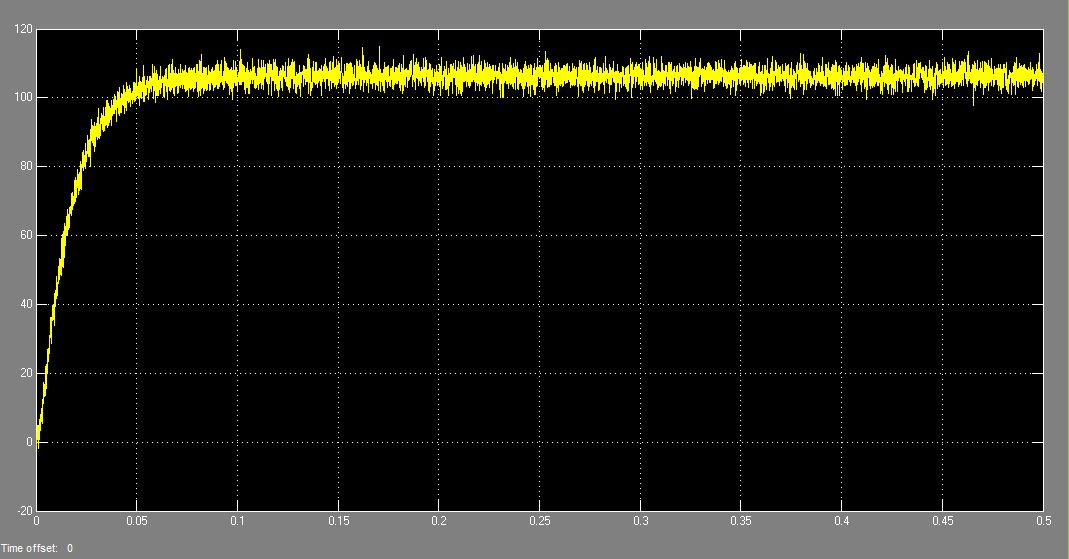
\includegraphics[width=.9\linewidth]{Simulacao_motor_excitado_por_degrau.jpg}
\caption{Simulação no Matlab da fução de transfêrencia do motor excitada por um degrau de 12.3 Volts}
\label{Simulcao matlab motor 1}
\end{figure}

\begin{figure}[h!]
\centering
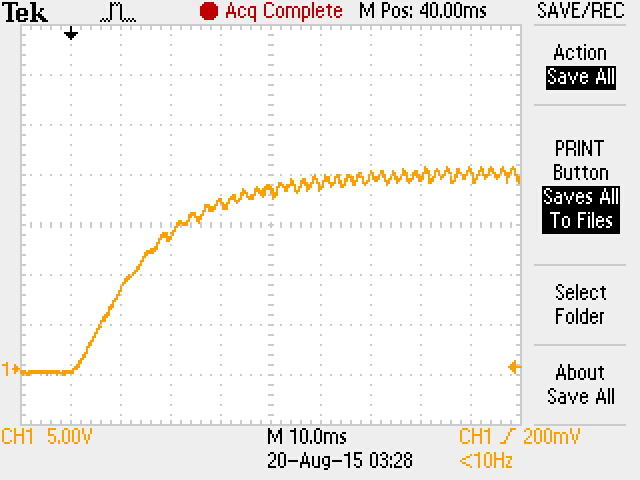
\includegraphics[width=.7\linewidth]{motor_osciloscopio.jpg}
\caption{Resultado da velocidade do motor segundo uma excitação degrau de 12.3Volts}
\label{Extracao de dados osciloscopio motor 2}
\end{figure}

Por meio do IDENT do matlab, descobriu-se qual era a função de transferência do motor, e é como se expressa na equação (\ref{FTM}) contando com o fato de que deve-se dividir o ganho da função pelo ganho do tacogerador, pois a velocidade foi obtida por meio do tacogerador, havendo, assim, sua influência.

\begin{equation}
\label{FTM}
G(s)_{motor}=\frac{343878,26}{(s-482,88)(s-66,93)}
\end{equation}

Uma vez definida a função de transferência do motor, cabe agora analisar o dispositivo que atuara fazendo o controle de velocidade do motor, dispositivo cujo nome é PWM (Pulse Widht Modulation) que será discutido no próximo tópico.

\subsection{PWM}

O controle baseado no principio de modulação por largura de pulso tem base teórica no fato de que a tensão média aplicada por uma onda quadrada é tanto maior quanto maior a largura do pulso em nível alto, e , desse modo, alterando a largura do pulso, pode-se alterar a potência entregue a planta.Abaixo encontra-se a verificação teórica da tecnica PWM consistindo em analisar a potencia de uma onda onda quadrada e verificando oque ocorre quando altera-se a largura do pulso.
\\
Lembrando que potência média de uma forma de onda é a integral dentro do período divido pelo período da mesma, como se segue na equação (\ref{Potencia media})

\begin{equation}
\label{Potencia media}
Potencia Media=\frac{1}{T}{}\int_{0}^{T}f(t)dt 
\end{equation}
\\

Como uma função quadrada com largura de pulso variável é definido por $y_{max}$ para $0\leq t\leq Dt$ e $y_{min}$ para $
Dt\leq t\leq T$, tem -se a seguinte expresão após a integração.

\begin{equation}
Potencia Media=Dy_{max}+(1-D)y_{min} 
\end{equation}
\\
Assim obserava-se que variando a largura do pulso, que na expressão consite no valor de D, tem-se uma maior potência para D=100\% e 0 de potência para D igual a 0\%.

\subsection{Aspecto Prático do PWM}
O dispositivo PWM também possui uma constante como função de trânsferência, e para levanta-la foi feira a seguinte experiência prática.Aplicou-se um sinal de PWM no motor e alterou-se a tensão de referência do mesmo, busncado verificar qual era a largura do pulso aplicando quando uma tensão era aplicada no PWM.Os valores verificados seguem na tabela (\ref{TabelaPWM}).

\begin{table}[h!]
\centering
\caption{Tabela com os valores de tensão aplicado no PWM (Vin), tempo em nivel lógico alto (Ton) Tensão de saída do PWM (Vout) constante do PWM (Kpwm)}
\label{TabelaPWM}
\begin{tabular}{|c|c|l|l|}
\hline
\multicolumn{1}{|l|}{Vin} & \multicolumn{1}{l|}{Ton} & Vout  & Kpwm  \\ \hline
1,94                      & 18us                     & 2,511 & 1,294 \\ \hline
3,86                      & 32us                     & 4,465 & 1,156 \\ \hline
5,96                      & 52us                     & 7,255 & 1,217 \\ \hline
8,01                      & 68us                     & 9,488 & 1,184 \\ \hline
10                        & Ton=T                    & 12    &  1,2     \\ \hline
\end{tabular}
\end{table}

A constante do PWM é dada pela razão $K_{pmw}=\frac{V_{out}}{V_{in}}$.Seu valor, por meio da tabela, verifica-se que é por volta de 1,2.

Desse modo tem-se a configuração do tacogerador, e sua função de transferência, o mesmo para o motor e para o pwm.Agora resta fechar a malha do sistema e definir os parametros de controle, para que assim seja implementado o controle do motor.

\section{Conclusão Malha Aberta}  
% The block diagram code is probably more verbose than necessary
\begin{figure}[h!]
\centering
\begin{tikzpicture}[auto, node distance=2cm,>=latex']

    % We start by placing the blocks
    \node [input, name=input] {};
    \node [sum, right of=input] (sum) {};
    \node [block, right of=sum] (controller) {Controlador};
    \node [block, right of=controller, pin={[pinstyle]above:Ruido},
            node distance=3cm] (system) {Motor};
    % We draw an edge between the controller and system block to 
    % calculate the coordinate u. We need it to place the measurement block. 
    \draw [->] (controller) -- node[name=u] {$u$} (system);
    \node [output, right of=system] (output) {};
    \node [block, below of=u] (measurements) {Sensor};

    % Once the nodes are placed, connecting them is easy. 
    \draw [draw,->] (input) -- node {$r$} (sum);
    \draw [->] (sum) -- node {$e$} (controller);
    \draw [->] (system) -- node [name=y] {$y$}(output);
    \draw [->] (y) |- (measurements);
    \draw [->] (measurements) -| node[pos=0.99] {$-$} 
        node [near end] {$y_m$} (sum);
        
 
\end{tikzpicture}
\caption{Esquema em Diagrama de Blocos do Controle do Motor}
\label{malha fechada}
\end{figure}  
        
A representação esquemática acima ilustra o circuito dejesado para que se faça  o controle do motor.Uma vez que tenha-se em mãos os parametros que definem o motor, o tacogerador, identificado como sensor, bastando agora definir os parametros do controlador.
Nesta primeira parte do curso fica a conclusão de que o controle de um sistema necessita do conhecimento da função de transferência dos componentes que compõe o sistema, sendo, no presente caso, o motor, a planta, o tacogerador , sendo o sensor, e o dispositivo controlador PWM.Na próxima etapa a busca será por encontrar uma controlador via malha fechada do sistema, como ilustrado na figura (\ref{malha fechada}) para assim estabelecer parametros de controle que definiram o projeto.

\section{Controle e Ajustes em Malha Fechada}
Verificou-se que os requisistos de controle em malha fechada, considerando controle em malha aberta, apenas proporcional, não atende os requisistos de controle, sendo eles erro de regime permanente menor que 5\%, tempo de acomodação metade do de malha aberta e overshoot  de no máximo 4.6\%.Assim se faz necessário implementar outros modos de controladores analógicos disponíveis, tais como PI ou PID.\\
O controle PID não faz juz ao controle do motor, pois, por ter um bloco derivador, este irá elevar a saída do controlador a valores inaceitaveis, afinal há um grande ruido por parte da reposta do motor como pode ser visto na figura (\ref{Extracao de dados osciloscopio motor 2}).Assim se faz a tentativa do controle por meio dos controladores PI, que apenas alteram o sinal de entrada de modo integral e proporcional.O bloco controlador integral zera o erro de regime permanente e o controle proporcional, junto ao integrador, faz com a resposta transiente seja também alterada, bastando ajustar esses parâmentros afim de alcançar os requesitos exigidos de controle.
\subsection{Controladore PI}
Os modos de controle em malha fechada consistem em realimentar a saída que por sua vez  passa por um controlador e é passado para a planta novamente.Um fator crucial, é que o erro e provindo da resposta instatânena da planta em comparação com a entrada é repassado ao controlador e subsequentemente para a planta, mantendo o ciclo até que os requesitos de controle sejam atendidos.\\
Abaixo, na equação (\ref{equacaoPI}) encontram-se as equações que regem o funcionamento do circuito PI, que será utilizado neste projeto.Obsetava-se que e(t)  é o erro que provem entre a comparação da entrada com a saída.
 \begin{equation}
 u(t)=Kpe(t)+ K_i\int_{a}^{t}e(t)dt
 \label{equacaoPI}
 \end{equation}
 
 A figura (\ref{esquematicoPI}) ilustra o esqumático em blocos de um controlador PI.
 
\begin{figure}[h!]
\centering
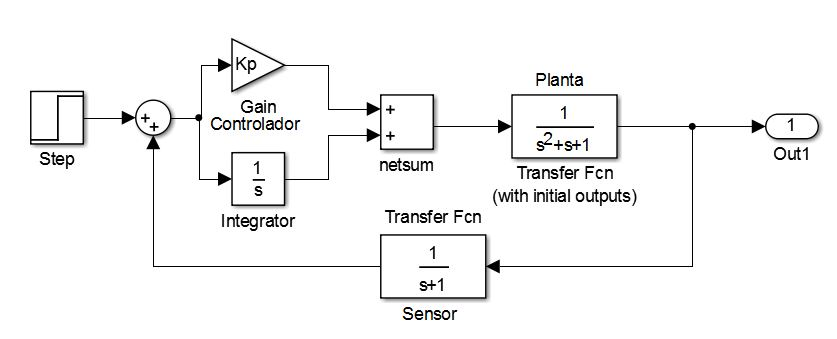
\includegraphics[width=.7\linewidth]{Pi_controler.jpg}
\caption{Esquemático do controle PI Simulink}	
\label{esquematicoPI_simulink}
\end{figure}

Por meio do Matlab é possível encontrar quais são os valores que devem ser colocados no controlador PI em função dos parametros desejaveis de controle, isso feito por meio da ferramente RLtool.Após obtidos esses valores coloca-se no simulink no referido bloco PI e efetua-se a simulação.Os resultados bem como o bloco esquemático do simulink encontra-se nas figuras (\ref{Malha_fechada_simulink}, \ref{Simulacao_malha_fechadaPI}) logo abaixo.

\begin{figure}[h!]
\centering
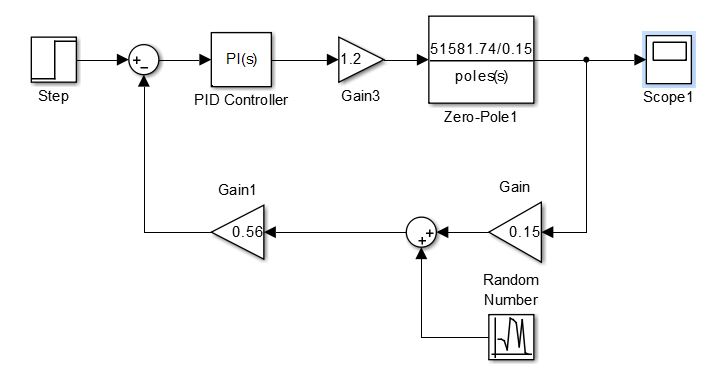
\includegraphics[width=.7\linewidth]{Malha_fechada_simulink.jpg}
\caption{Esquemático De Malha Fechada no Simulink}	
\label{Malha_fechada_simulink}
\end{figure}

\begin{figure}[h!]
\centering
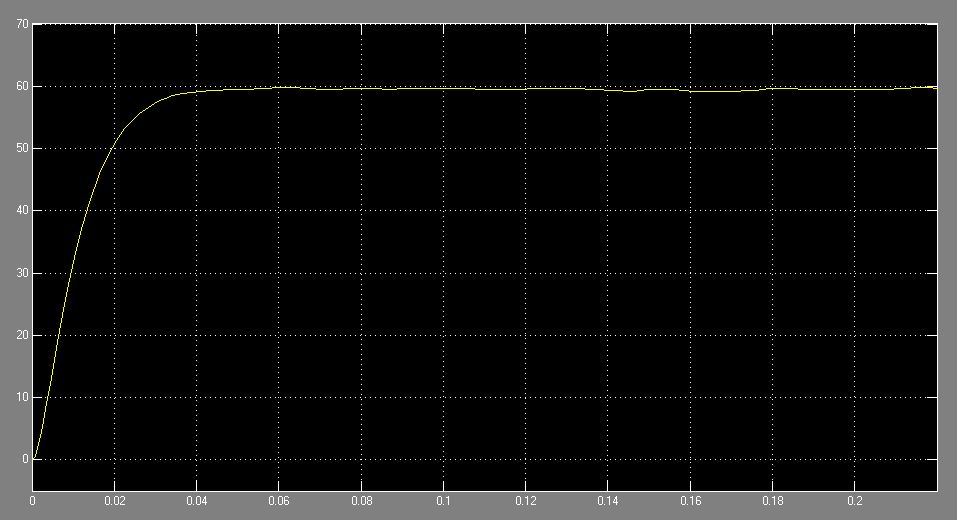
\includegraphics[width=.7\linewidth]{simulacao_malha_fechada.jpg}
\caption{Resultado da Simulação em Malha Fechada Com Controle PI}	
\label{Simulacao_malha_fechadaPI}
\end{figure}

\section{Implementação Do Controlador PI}
Partindo dos valores fornecidos para os ganhos $K_p$ e $K_i$ que foram 1,10506 e 82,184 pode-se calcular os valores das resistências e capacitores que irão encontra-se nos amplicadores proporcionais e integradores, basntando que seja satisfeita a razão de ganho em ambos amplificadores.Abaixo, na figura (\ref{Amplificador_PI}) encontra-se a configuração do sistema com os amplificadores operaionais atuando como proporcionais e integradores.Os amplificadore utilizados para efetuar o processo foi o UA741.

\begin{figure}[h!]
\centering
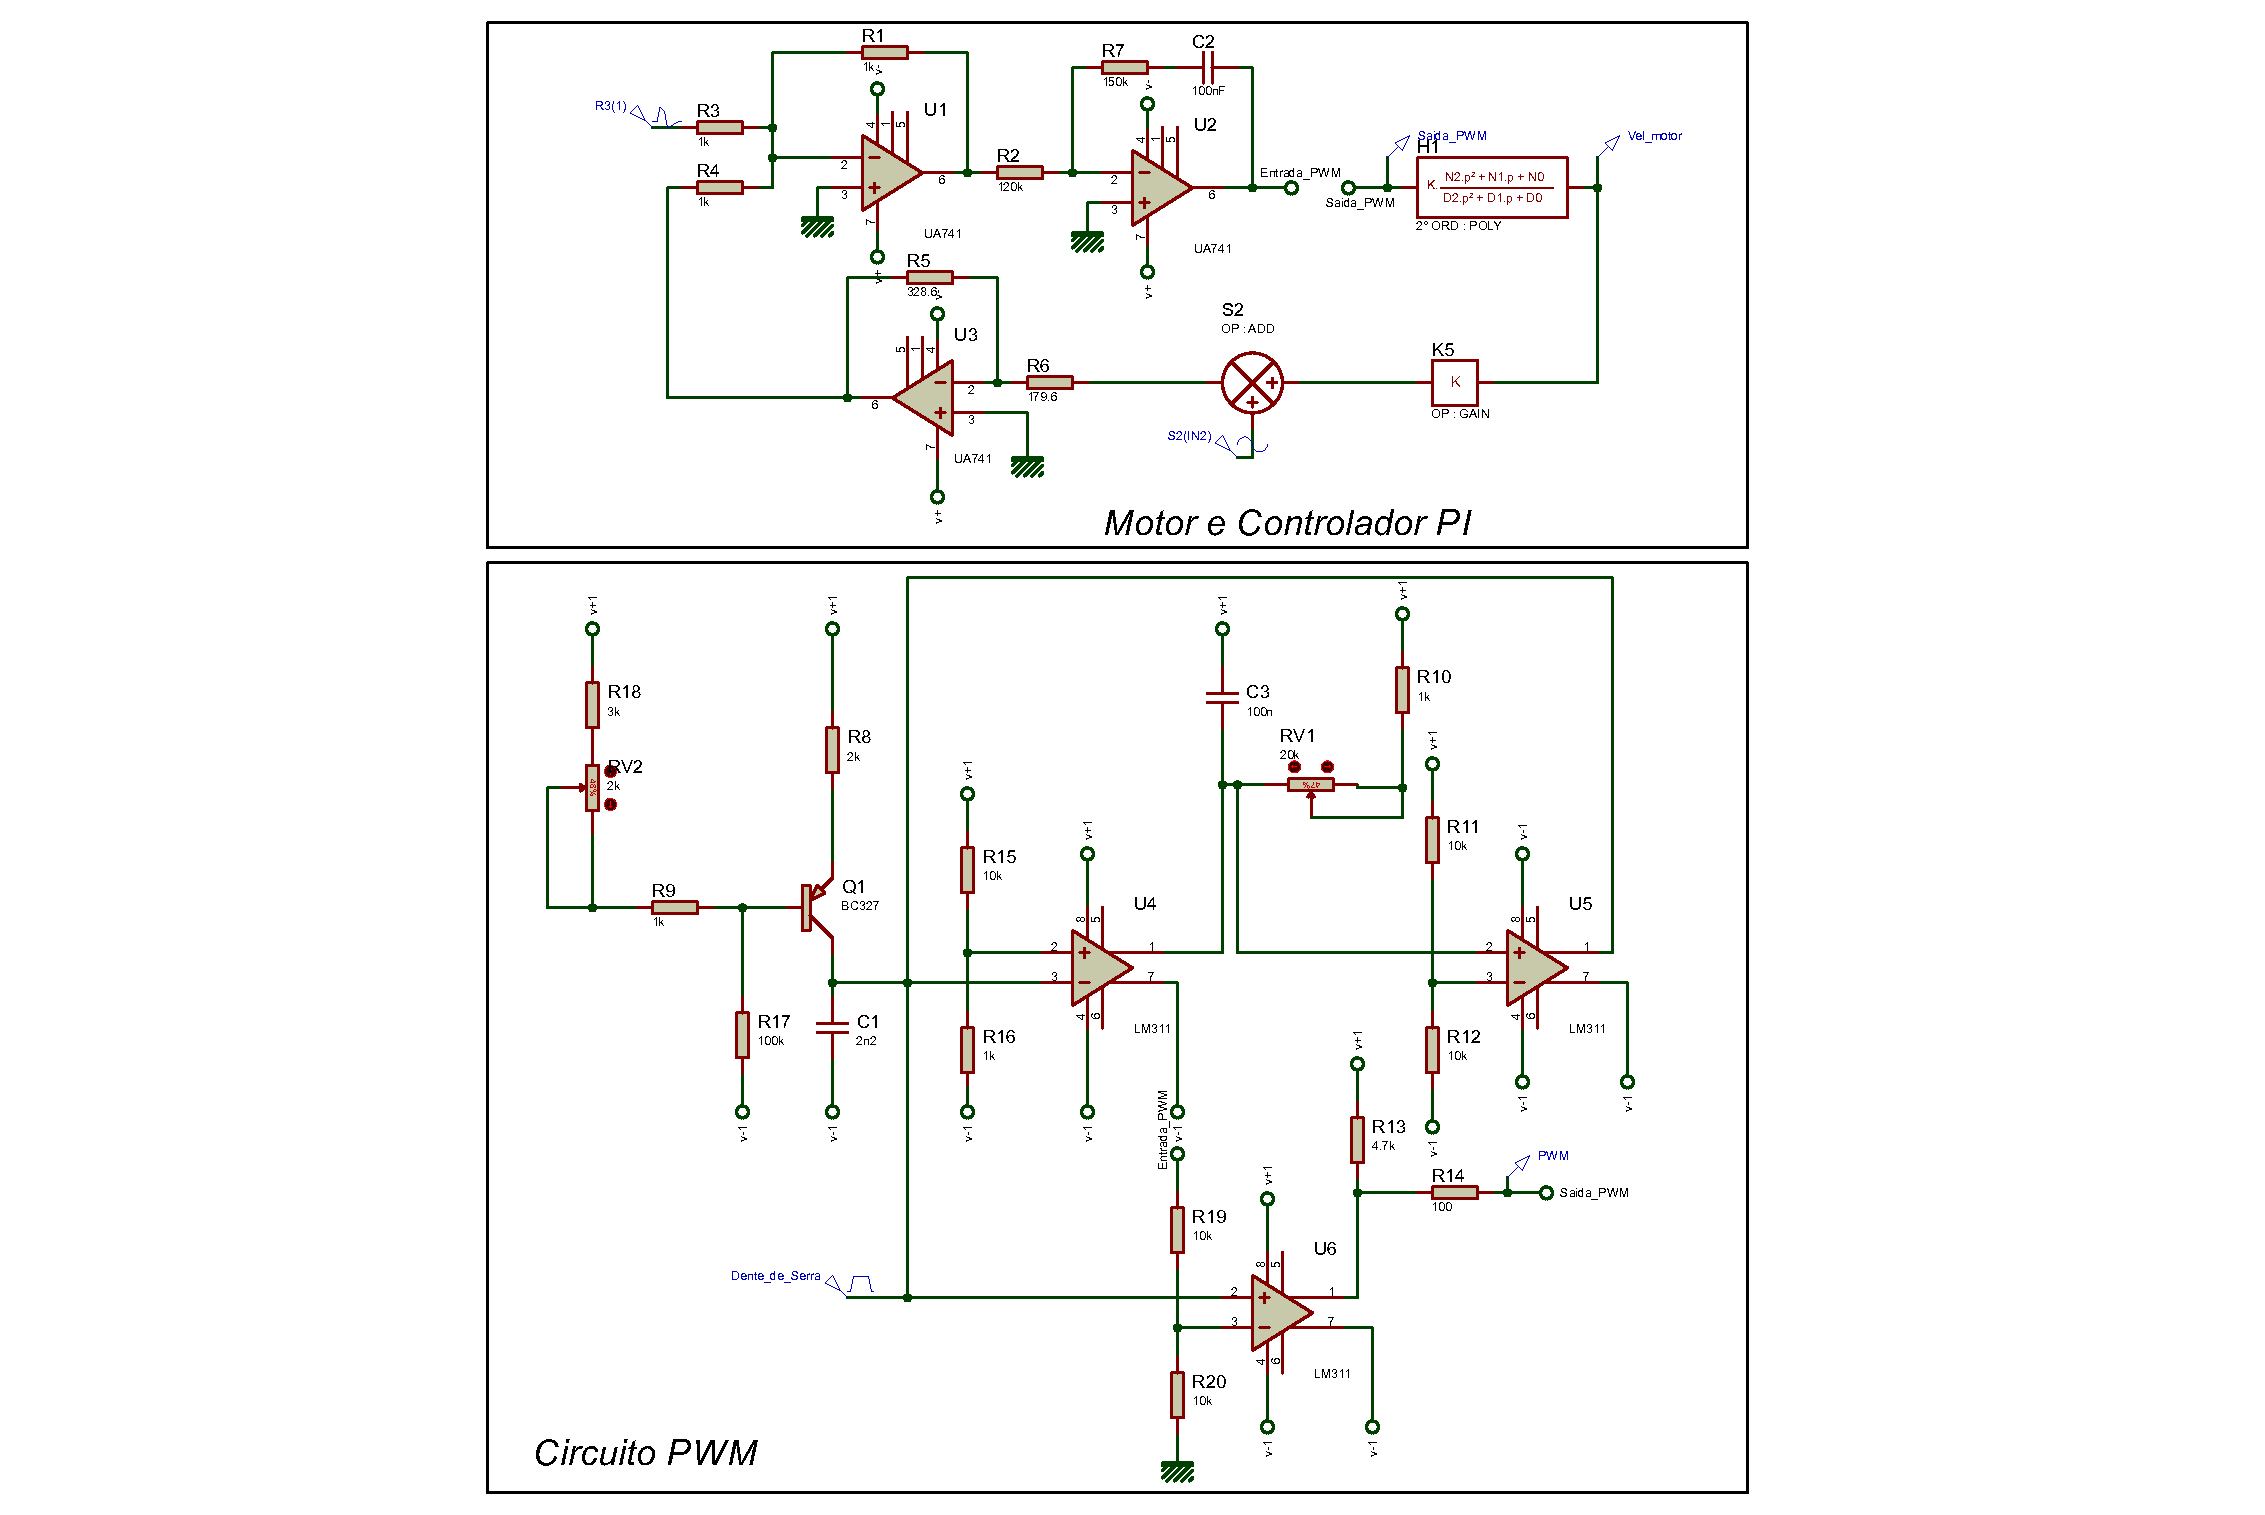
\includegraphics[width=.9\linewidth]{amplificador.pdf}
\caption{Circuito com os Amplificadores Operacionais Atuando Como Porporcional e Integrador, além do PWM}	
\label{Amplificador_PI}
\end{figure}

Assim o controlador PI deve ser implementado como na figura (\ref{Amplificador_PI}) substituindo o bloco de ganho 1.5 pelo dispositivo PWM.\\
O circuito fora implementado em bancada juntamente com o PWM e a resposta obtida encontra-se na figura (\ref{Resultado}) logo abaixo.Verifica-se que o resultado se equipara ao simulado, que se econtra na figura (\ref{malha_fechada_simulacao}), valendo todos os procedimentos teóricos utilizados neste experimento.

\begin{figure}[h!]
\centering
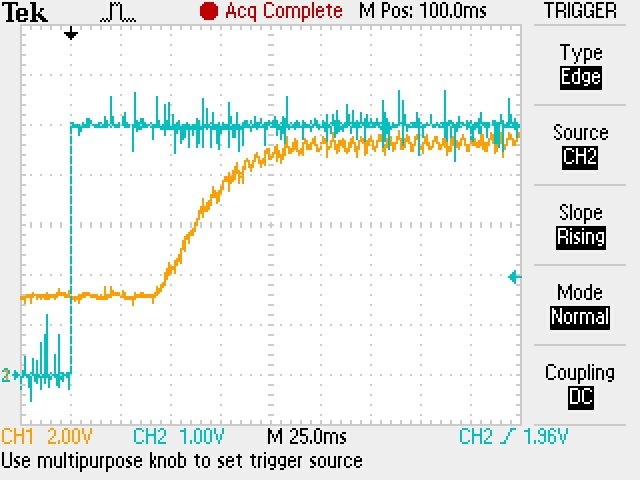
\includegraphics[width=.6\linewidth]{Resultado_experimento.jpg}
\caption{Resultado da Implementação do Controlador PI}	
\label{Resultado}
\end{figure}

\begin{figure}[h!]
\centering
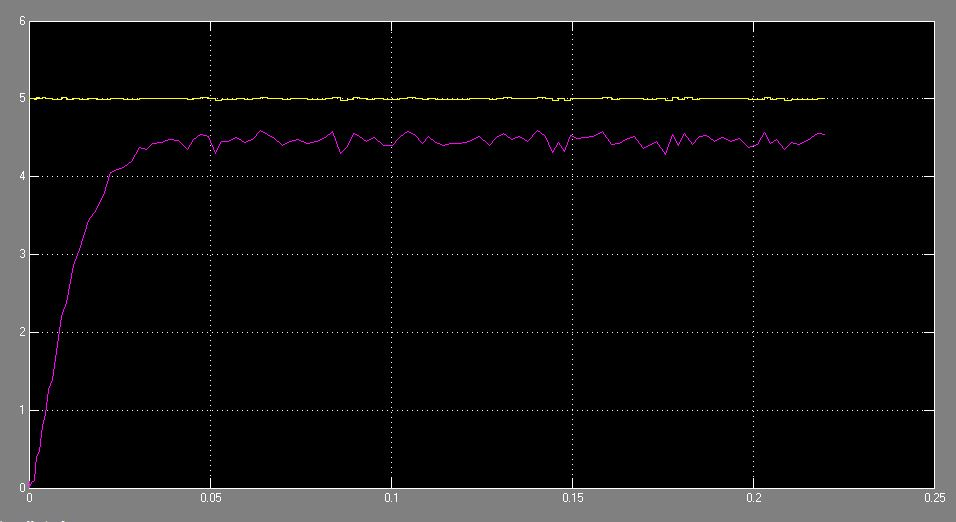
\includegraphics[width=.9\linewidth]{simulacao_malha_fechada_osciloscopio.jpg}
\caption{Resultado da da Simulação do Controlador PI.}	
\label{malha_fechada_simulacao}
\end{figure}

Como pode-se observar a ponta de prova do osciloscópio estava na saida do tacogerador, oque faz com que a mesma seja dividida pela constante de amplificação do mesmo, que é por volta de 0.15.Assim, sendo esperado que a velocidade do motor em malha fechada tivesse um valor próximo de 60rad/s para um degrau de 5 Volts foi alcaçado, pois, como verifica-se a tensão emitida pelo tacogerador foi de 9.52 Volts, oque, dividido por 0.15 gera um valor de 63,46 rad/s, condizendo com as previsões de simulação, como pode ser visto na figura (\ref{Simulacao_malha_fechadaPI}).

 \section{Verificação dos Critérios de Desempenho em Malha Fechada e Aberta e Comparações.} 
 O objetivo de controle era fazer com que o overshoot máximo não ultrapasasse 4.6\%, que o erro de regime permanente fosse menor que 5\% e o tempo de acomodação fosse metade do de malha aberta.Abaixo enontra-se a exlpicação para esses termos.

  \begin{itemize}  

        \item Overshoot: Trata-se do valor que a resposta assume quando dá o primeiro salto de tensão na mesma, excedendo o valor de estado estacionário ou regime permanente.Não houve overshoot em ambas as respotas, malha aberta e fechada, sendo assim não há comparação a fazer, apenas fica o fato que este critério de desempenho foi alcançado, ou ao menos não houve a necessidade de controlá-lo.

        \item Erro de Regime Permanente: Trata-se da diferença que há entre o valor da entrada e da saida em regime permanente, considerando a malha fechada.Por haver um controlador integrador, o erro é para tender a zero, porém isto limita o tempo de acomodação, havendo então um balanço entre esses dois parâmetros de controle.Como pode ser visto na figura (\ref{erro_regime}) o erro tende a zero com o tempo, e por meio de média aritimética verifica-se que o erro é da ordem de 0.68 sendo 6.8\% , quase atendendo ao critério de performance espercifica, que está na faixa de 5\%.Porém, deve-se enfatizar que o o sinal de saída possui um grande ruido, o que afeta o sistema no seu estado estacionário, justificando o erro de regime calculado. 
        
        \item  Tempo de acomodação:Trata-se do tempo que sistema leva para deixar de variar a sua resposta devido ao overshoot em um intevalo de amplitude de -5\% a +5\% do valor de regime.Como não houve overshoot no sistema, pode-se dizer que este fator foi alcançado. 
 
    \end{itemize}
               
\begin{figure}[h!]
\centering
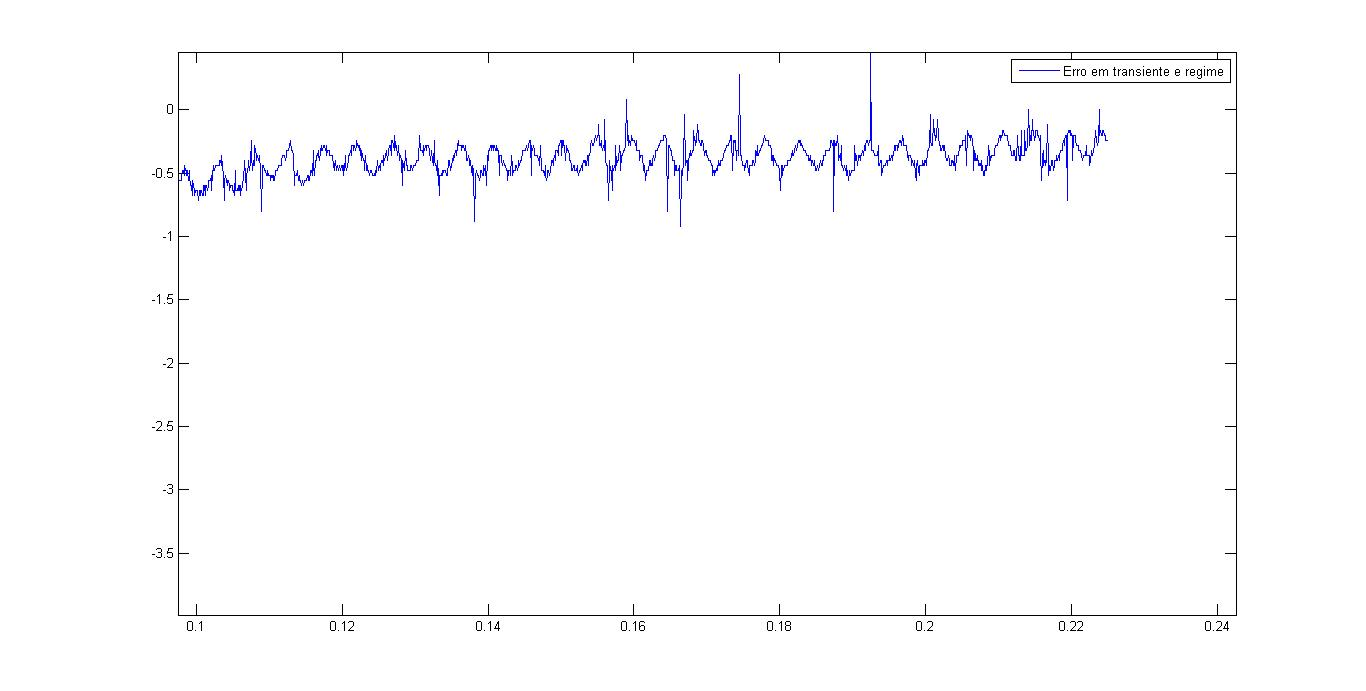
\includegraphics[width=\linewidth]{Erro_de_regime_permanente.jpg}
\caption{Erro de Regime Permanente.}	
\label{erro_regime}
\end{figure}

\newpage

\section{Tratamento dos Dados Para a Obteção da Velocidade}
Os dados obtidos experimetalmente presente na figura (\ref{Resultado}) e na simulação presente na figura (\ref{malha_fechada_simulacao}) representam a tensão gerada no saida do tacogerador, sendo assim não representam a velocidade de rotação do motor, afinal o ganho do tacogerador é 0.15.Assim, há a necessidade de se dividir a resposta por 0.15 para obter a velocidade de rotação, esperando que o resultado seja confome mostrado na simulação da figura (\ref{Simulacao_malha_fechadaPI}).\\
Abaixo, na figura (\ref{vel_rotacao_dados}) pode-se observar que a simulação encontra-se em perfeita ligação com os dados apresentados nas figuras que representam a velocidade de rotação do motor.

\begin{figure}[h!]
\centering
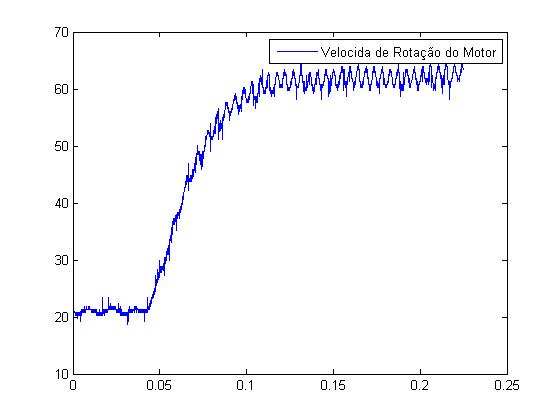
\includegraphics[width=.6\linewidth]{Velocidade_real_do_motor_experimental.jpg}
\caption{Velocidade de Rotação do Motor em RPM}	
\label{vel_rotacao_dados}
\end{figure}

\section{Conclusões}
Pode-se ver que as simuações feita no matlab feicaram com boa precisão com relação aos experimentos, mostrando grande fidelidade do software mesmo com operações complexas, como ajunstar os pólos em malha fecahda por meio do RLTOOL.Houveram falhas minimas, menos de 1\% na  verificação do erro de regime permanente com relação ao epxperimento, porêm é aceitálvel pois há um grande ruído na saida do tacogerador.Outro fato a se observar é que a montagem do cirucito na prática deve obedecer a lei de colocar resistências de alto valor para fazer com que os amp-ops funcionem corrtamente, pois há problemas com relação  impedância de entrada dos mesmos com baixos valores de resistência.
Por fim verificou-se a necessidade de se colocar um capacitor juntoa saída do tacogerador com a entrada do circuito PI, pois os ruídos provindo do motor estavam impedindo a captação dos sinais de velocidade.\\

 \newpage 

\section{Apêndice:Simulação no Proteus do Sistema Motor DC}
O software proteus, oferecido pela empresa Labcenter Electronics, não é gratuito, apesar de haver a versao demo disponível no site da fabircante.Possui diversos componentes tanto na área analógica quanto digital, estando muito deles disponíveis para simulação.Há componentes ideais, que fazem seu principio sem parametros de limitação, e componentes especificado por fabricantes, havendo também a possibilidade de se criar componentes, tanto em esquemático quanto em PCB (Printed Circuit Board) para fins de construção do esquemático produzido.Por enquanto o que se vê de diferencial é a presença de componentes digitais, e isso não se restringe a portas lógicas e flip-flops como encontra-se presente em diversos softwares de simulação, mas também com conversores AD e DA de vários fabricantes e micrcontroladores programáveis de diversos fabricantes, indo desde de ARM a outros menos robustos como a famosa família de controladores MCU8051.Display de sete segmentos e de cristal liquido também encontram-se presentes, permitindo a simulação a conjunta dos componentes citados.Memórias também encontram-se disponiveis para simulção e esquemático e simulação conjunta com outros periféricos.Em fim, fica a critéirio do projetista como utilizar os vários componentes presentes no simulador.\\
Um outro fato que leva a utilização do proteus, é a relação que exite entre suas duas interface ISIS e ARES, que permite a construção do projeto esquemático do ISIS  apenas transportando para o ARES com as ligações entre componentes já executada, oque é comum em softwares de PCB.Oque diferencia  o proteus é que o esquemático já possui sua simulação feita, assim o PCB só é executado quando o esquemático estiver funcionando, garantindo de primeira a construção do circuito.A figura (\ref{PCB_esquematico}) ilustra essa vantagem.\\

\begin{figure}[h!]
\centering
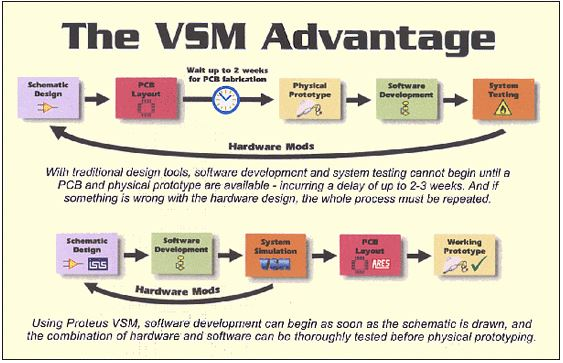
\includegraphics[width=.5\textwidth]{Simulcao_proteus_esquematico_PCB.jpg}
\caption{Simulação Proteus e Matlab e Dados Obitdos Experimetalmente \cite{labcenter}}
\label{PCB_esquematico}
\end{figure}

\section{Revisão de trabalhos feito no Proteus}
Apesar não ser tão extensa quanto a bibliografia de trabalhos que usam o matlab, o proteus tem uma gama de artigos publicados que fazem o seu uso considerável, principalmente quando há a utilização de microcontroladores no sistema em questão, afinal uma grande potencilalidade do proteus é a presença de vários microcontroladores e periféricos, sendo que alguns artigos defendem o uso do proteus como ferramenta para o ensino de microcontroladores\cite{Ensino_proteus_uc}\cite{proteus_educacao}.A presença de vários tipos de motores provem a possibilidade de simula-los, como pode ser visto no seguinte trabalho\cite{motor_brushless}.Controle de cargas  e sistemas de potência baseado em microcontroladores PIC (Programmable Integrate Circuit) também encontram-se desenvolvidos\cite{busca_de_maxima_potencia_com_sistemas_microcontrolados}.Simulação do  uso de pesticidas emitidos por meio de circuitos microcotrolados\cite{pesticida}.A simulação e construção de display de leds em caracteres de chineses também já foi implementada \cite{caracteres_chineses}e outras utilidades utilizando displays \cite{simulacao_led_proteus_display}.\\
Trabalhos mais impactantes também foram feitos, que utlizam praticamente somente o proteus como software de simulação, como exemplo tem-se a construção de um microcomputador \cite{contrucao_microconputador_proteus}, o controle de carga (explicar melhor) \cite{controle_de_carga}.A construção de um termostato \cite{termostato} o controle de temperatura e humidade baseado no proteus \cite{controle_de_temperatura} avanços na tecnologia de pizoeletrico \cite{pizoeletrico}, a construção de um voltimetro digital por meio de micrconcontroladore \cite{voltimetro_digital}, busca de máxima portência utilizando sistemas micrcontrolados \cite{busca_de_maxima_potencia_com_sistemas_microcontrolados} e muitos outros trabalhos que utilizam diretamente e indiretamente o proteus como simulador.

\section{Simulações em Malha aberta}
Primeiramente as simulações visam verificar os resultados dos softwares , proteus e matlab, com relação aos dados reais e a ambos e entre si.Na figura (\ref{dados reais e simulacao}) encontra-se os resultados da simulação em malha aberta feita com a função de transferência do motor,bem como a curva obitida experimentalmente e, na figura (\ref{erro Malhaaberta}) encontra-se o erro obtido em relação as duas simulações com os dados obtidos experimentalmente.Como pode-se observar o erro é tolerante em ambas as simulação.

\begin{figure}[h!]
\centering
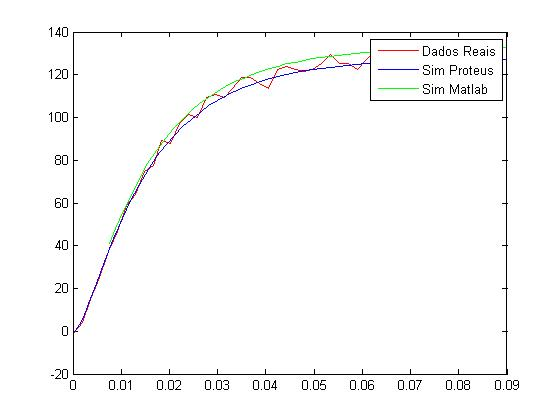
\includegraphics[width=.7\textwidth]{Dados_reais_matlab_proteus_malha_aberta.jpg}
\caption{Simulação Proteus e Matilab e Dados Obitdos Experimetalmente}
\label{dados reais e simulacao}
\end{figure}

\begin{figure}[h!]
\centering
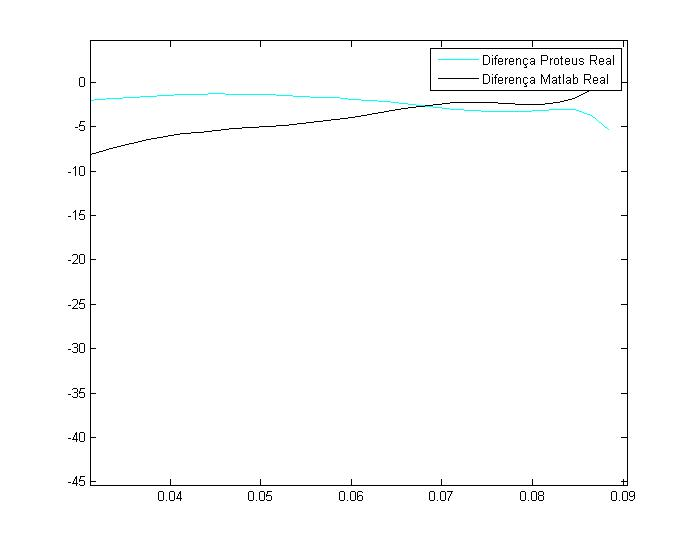
\includegraphics[width=.7\textwidth]{erro_malha_aberta.jpg}
\caption{Erro Com Relação aos Dados Reais da Simulação no Proteus e Matlab em Malha Aberta}
\label{erro Malhaaberta}
\end{figure}

Assim, verifica-se que ambas as simulações obtiveram erros razoáveis com os dados obitidos experimentalmente.Porém, cabe salientar que foi usado no proteus os blocos de função de transferência, que não é seu ponto forte, afinal não há uma grande gama de funções.No que diz respeito a simulação do controle do motor em malha fechada, caberá o uso de componentes reais do Proteus, sendo este seu ponto forte.Isto é conteúdo dos próximos tópicos.

\newpage

\section{Simulações do Controle em Malha Fechada.}
A simulação foi realizada no software Proteus utilizando os componentes e resistências que compõem o controlador, utilizando blocos para representar o PWM e o ganho do tacogerador, além da planta do motor.A figura (\ref{Circ_proteus}) ilustra a construção feita.

\begin{figure}[h!]
\centering
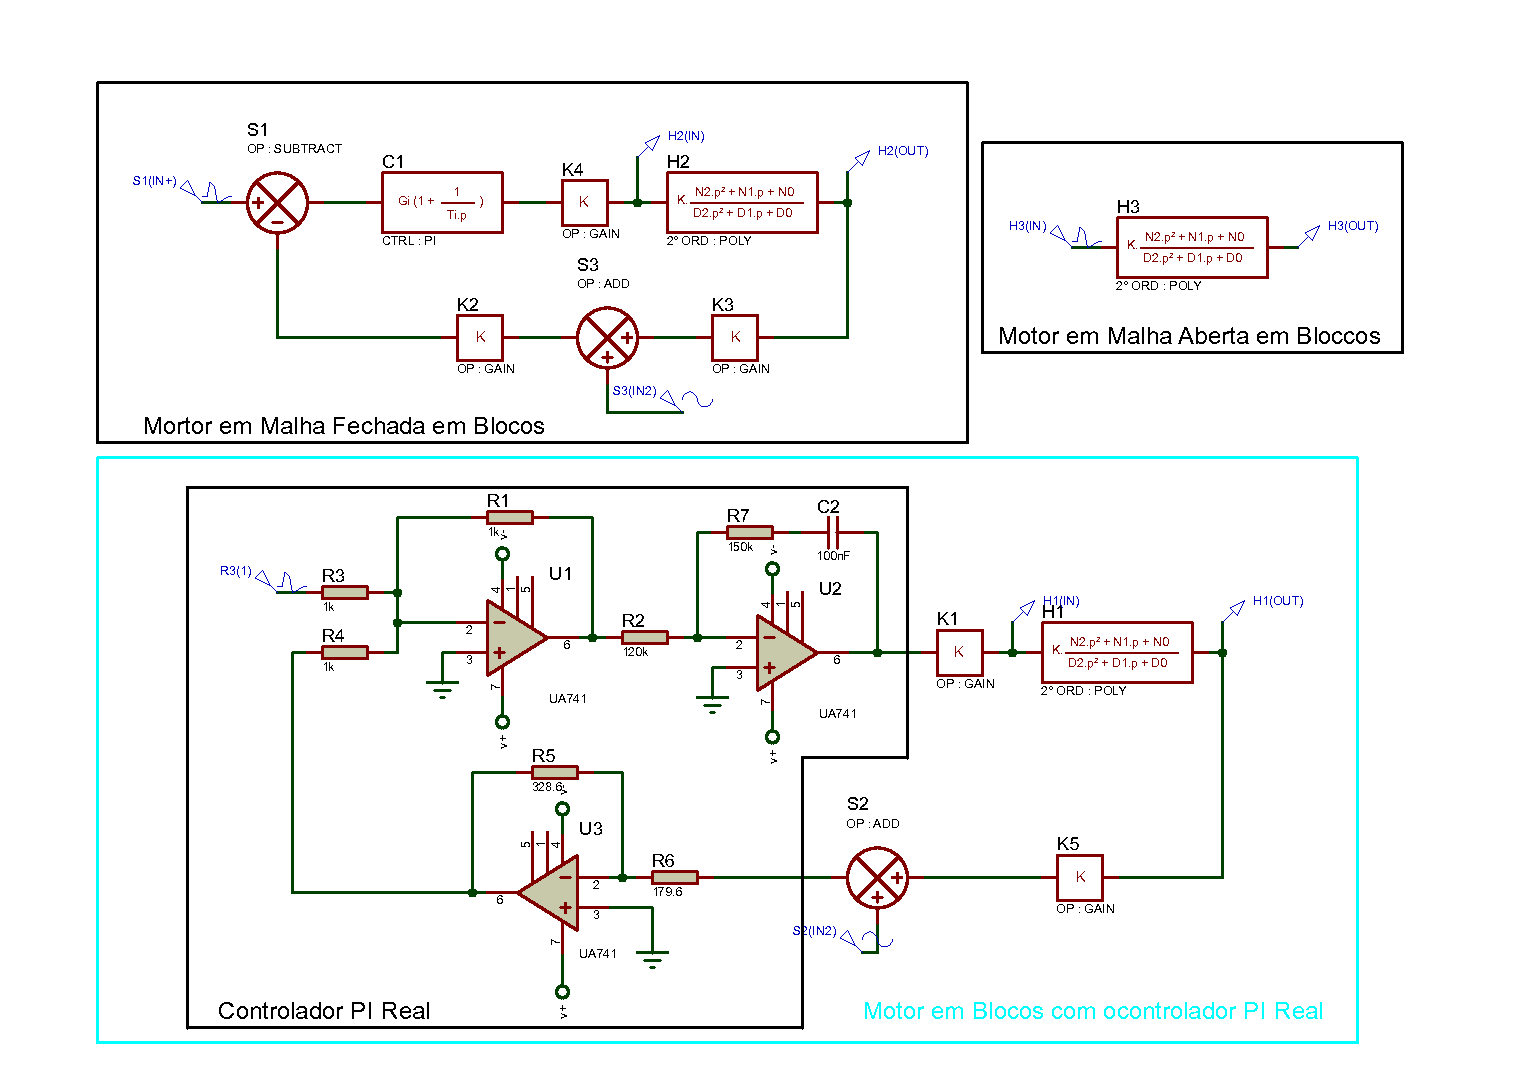
\includegraphics[width=.9\textwidth]{circuito_proteus.pdf}
\caption{Estrutura Simulada no Proteus com os Componentes Reais do Controlador}
\label{Circ_proteus}
\end{figure}

Foram feitas as simulações nos softwares Matlab e Proteus e plotadas juntamente com o intuito de verificar a precisão das simulações nos softwares, principalmente no proteus, por ser de menor reputação.A resposta real também foi plotada para verificar a precisão.Tal construção de simulações encontra-se na figura abaixo (\ref{sim_pro_mat}).


\begin{figure}[h!]
\centering
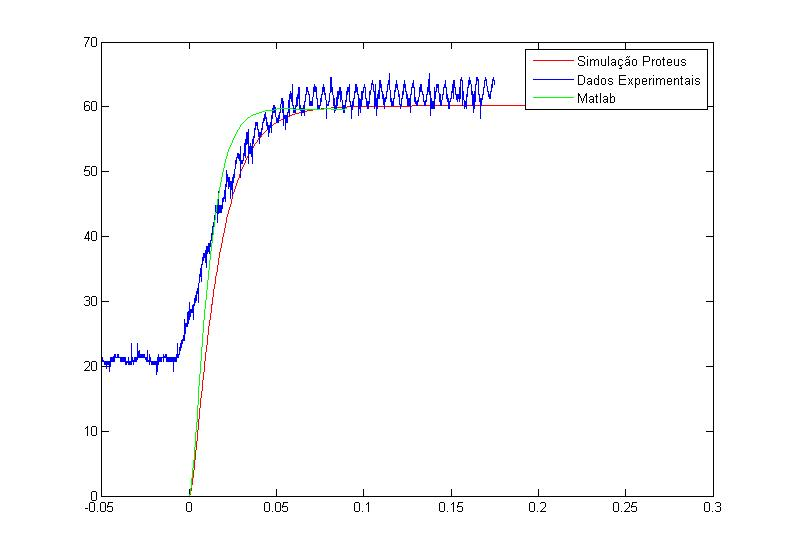
\includegraphics[width=.7\textwidth]{Comparacao_mat_pro_real_m_fechada.jpg}
\caption{Estrutura Simulada no Proteus e Matlab e Dados Obtidos Experimentalmente}
\label{sim_pro_mat}
\end{figure}

Por meio das comparações feitas entre os simuladores e dados obtidos no laboratório, verifica-se que são confiáveis as simulações no proteus para blocos de controle e amp-ops.

\section{Simulação PWM no Proteus e Construção da Placa de Controle}
O PWM é uma construção essencial no controle do motor, e  seu funcionamento, no quesito de componentes analógicos, se da por meio da comparação da forma de onda de uma dente de serra com uma tensão de referência.Conforme varia-se a tensão de referência  varia-se o duty cycle do PWM.A figura (\ref{PWM}) explicita o circuito do PWM utilizado, sendo que a figura (\ref{Simulacao_PWM_Proteus1}) expressa a simulação do componente.A simulação foi realizada com uma tensão de entrada no valor de  5,96 Volts, gerando o duty cycle precisamente como mostra a tabela (\ref{Simulacao_PWM_Proteus1}) que é de valor 52us.

\begin{figure}[h!]
\centering
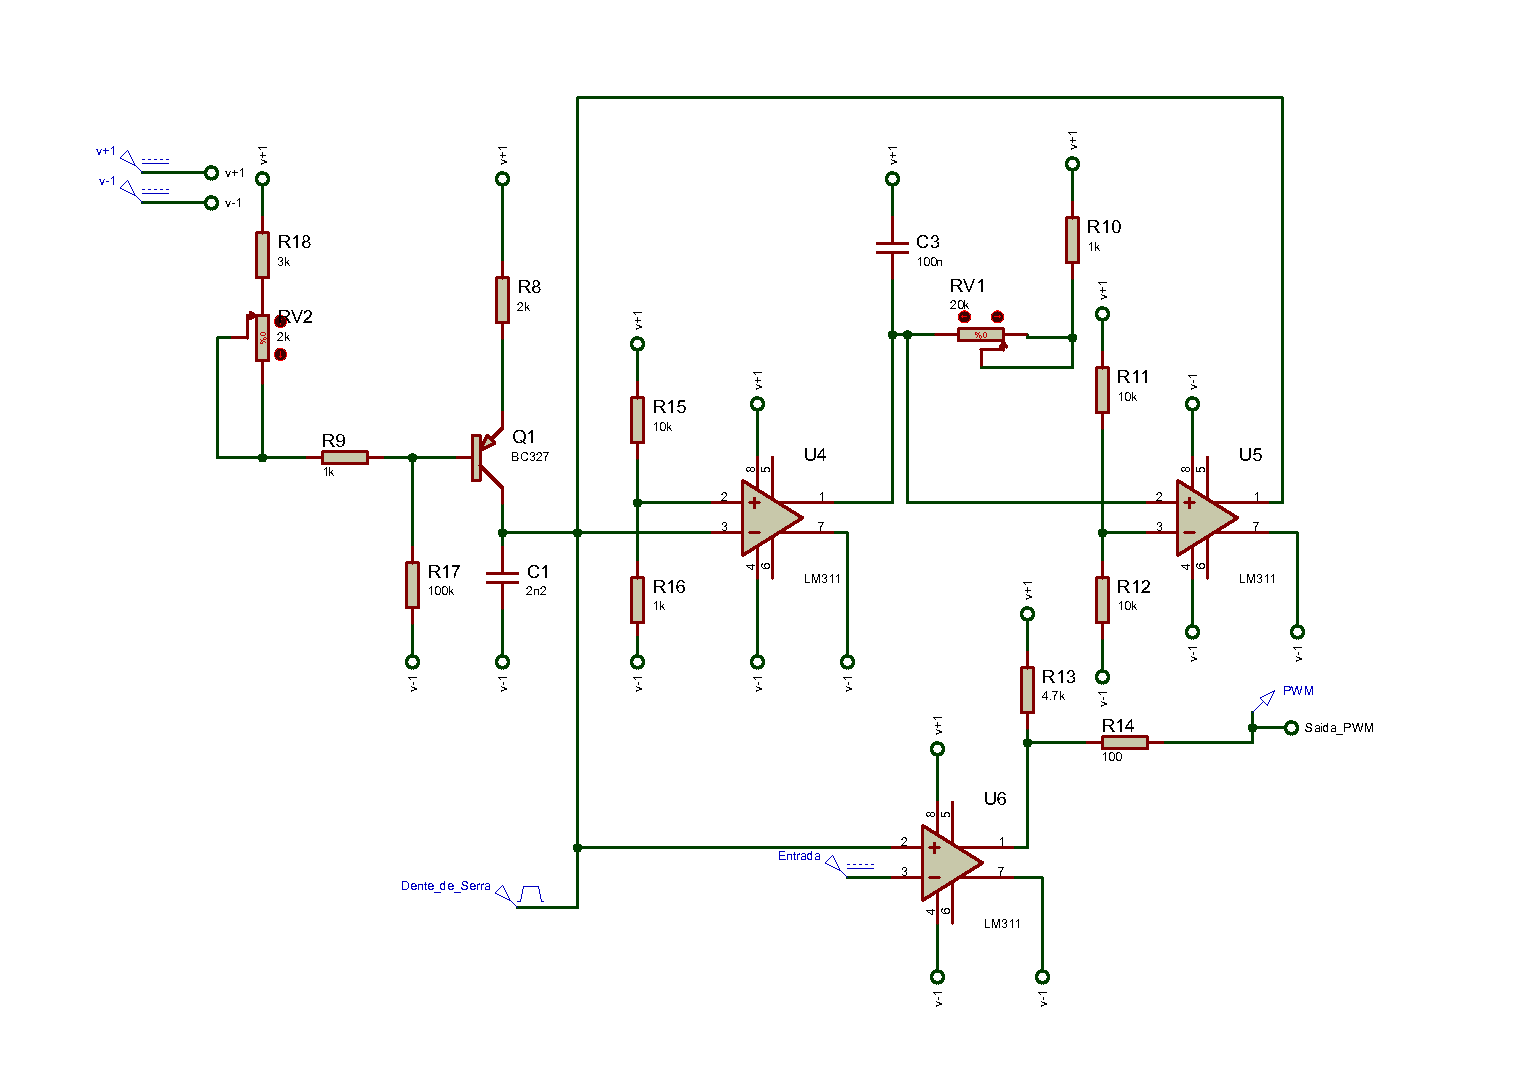
\includegraphics[width=.9\textwidth]{pwm.pdf}
\caption{Circuito PWM}
\label{PWM}
\end{figure}

\begin{figure}[h!]
\centering
\includegraphics[width=.5\textwidth]{simulacao_pwm_proteus.pdf}
\caption{Simulação do Circuito PWM da Figura Acima.}
\label{Simulacao_PWM_Proteus1}
\end{figure}

Como foi dito, o software Proteus possibilita a construção da placa de controle, além de sua simulação.Assim, a construção do projeto se dá quando todas as simulações estarem batendo com os resultados esperados, expresando essa vantagem como explicito na figura (\ref{PCB_esquematico}).O circuito em sua forma de simulação e renderização para o circuito real encontram-se nas figuras (\ref{PCB}), (\ref{Real}) abaixo.Com esta placa o controle do motor pode ser feito apenas conectando os elementos expressos na figura da placa real renderizada, sendo que  TC é a saida do Tacogerador, $+15V$ o 15 volts e $-15V$ o  menos 15 volts, $D_S$ a entrada dente de serra, se não se desejar colocar um componente que gere tal forma de onda na placa como o LM555 que é um dos CI's capaz de gerar essa forma  de onda, IN é tensão de referência para o PWMS e a saída do PWM que vai para o terminal do motor.

\begin{figure}[h!]
\centering
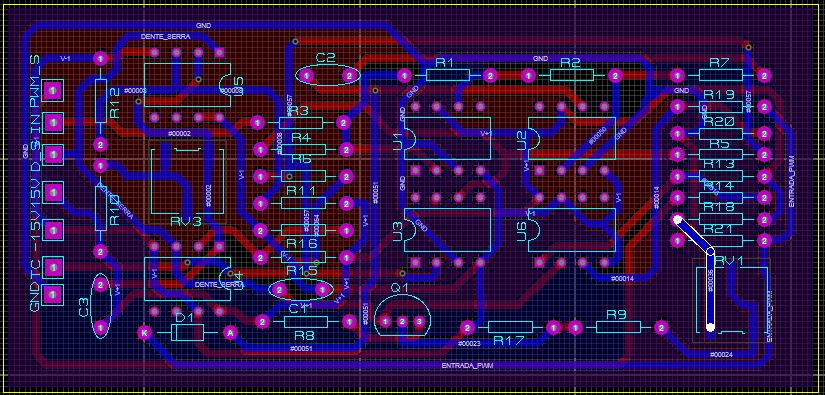
\includegraphics[width=.5\textwidth]{Proteus_PCB.jpg}
\caption{Imagem na Forma de PCB Construida no Software Proteus Ares}
\label{PCB}
\end{figure}

\begin{figure}[h!]
\centering
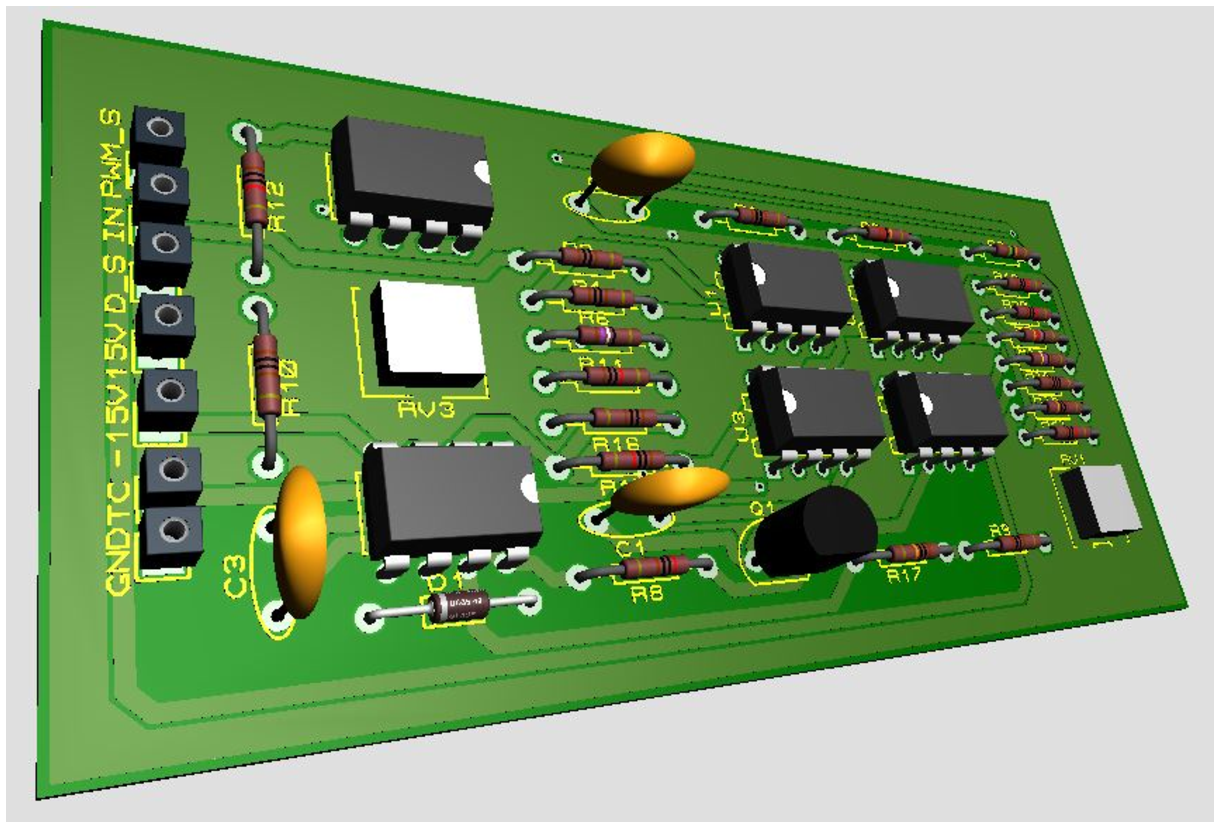
\includegraphics[width=.5\textwidth]{Proteus_Real.pdf}
\caption{Placa Renderizada do Circuito PCB Acima.}
\label{Real}
\end{figure}

\newpage

\section{Conclusão Simulação Proteus}
Como pode ser visto pela comparação das simulações, observa-se que o proteus possui grande fidelidade quanto a simulações, havendo pequena diferença entre a simulação no matlab, dados reais.O fato de poder-se simular e construir o circuito simulado é uma grande vantagem, afinal garante-se que o sistema terá o funcionamento desejado.Assim, conclui-se que tal software é um bom simulador para auxiliar em projetos de controle.

\newpage

\bibliography{Relatorio_Lab_de_Controle_de_Sistemas} 
\bibliographystyle{unsrt}
\end{document} 